\documentclass[14pt]{extbook}
\usepackage{multicol, enumerate, enumitem, hyperref, color, soul, setspace, parskip, fancyhdr} %General Packages
\usepackage{amssymb, amsthm, amsmath, latexsym, units, mathtools} %Math Packages
\everymath{\displaystyle} %All math in Display Style
% Packages with additional options
\usepackage[headsep=0.5cm,headheight=12pt, left=1 in,right= 1 in,top= 1 in,bottom= 1 in]{geometry}
\usepackage[usenames,dvipsnames]{xcolor}
\usepackage{dashrule}  % Package to use the command below to create lines between items
\newcommand{\litem}[1]{\item#1\hspace*{-1cm}\rule{\textwidth}{0.4pt}}
\pagestyle{fancy}
\lhead{Progress Quiz 7}
\chead{}
\rhead{Version C}
\lfoot{3510-5252}
\cfoot{}
\rfoot{Summer C 2021}
\begin{document}

\begin{enumerate}
\litem{
Write the equation of the graph presented below in the form $f(x)=ax^2+bx+c$, assuming  $a=1$ or $a=-1$. Then, choose the intervals that $a, b,$ and $c$ belong to.
\begin{center}
    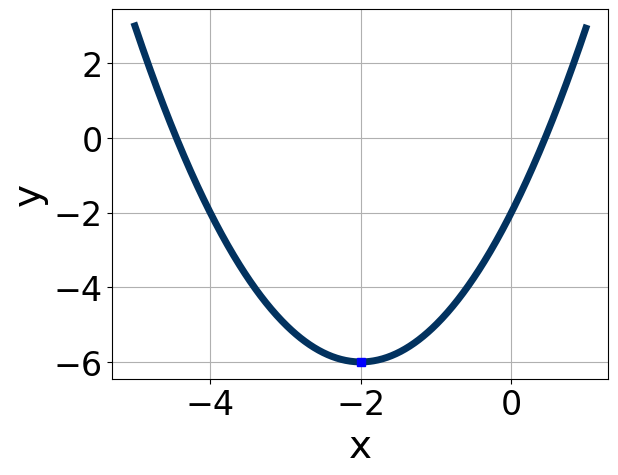
\includegraphics[width=0.5\textwidth]{../Figures/quadraticGraphToEquationC.png}
\end{center}
\begin{enumerate}[label=\Alph*.]
\item \( a \in [0.9, 1.7], \hspace*{5mm} b \in [-5, 1], \text{ and } \hspace*{5mm} c \in [-3, 2] \)
\item \( a \in [-1.1, -0.7], \hspace*{5mm} b \in [-5, 1], \text{ and } \hspace*{5mm} c \in [-12, -9] \)
\item \( a \in [0.9, 1.7], \hspace*{5mm} b \in [-5, 1], \text{ and } \hspace*{5mm} c \in [10, 11] \)
\item \( a \in [-1.1, -0.7], \hspace*{5mm} b \in [1, 6], \text{ and } \hspace*{5mm} c \in [-12, -9] \)
\item \( a \in [0.9, 1.7], \hspace*{5mm} b \in [1, 6], \text{ and } \hspace*{5mm} c \in [-3, 2] \)

\end{enumerate} }
\litem{
Solve the quadratic equation below. Then, choose the intervals that the solutions $x_1$ and $x_2$ belong to, with $x_1 \leq x_2$.\[ 25x^{2} -60 x + 36 = 0 \]\begin{enumerate}[label=\Alph*.]
\item \( x_1 \in [29.89, 30.07] \text{ and } x_2 \in [28.82, 30.39] \)
\item \( x_1 \in [0.29, 0.4] \text{ and } x_2 \in [2.8, 5.36] \)
\item \( x_1 \in [0.98, 1.27] \text{ and } x_2 \in [0.98, 1.24] \)
\item \( x_1 \in [0.5, 0.69] \text{ and } x_2 \in [2, 2.82] \)
\item \( x_1 \in [0.18, 0.24] \text{ and } x_2 \in [5.82, 8.14] \)

\end{enumerate} }
\litem{
Factor the quadratic below. Then, choose the intervals that contain the constants in the form $(ax+b)(cx+d); b \leq d.$\[ 54x^{2} -57 x + 10 \]\begin{enumerate}[label=\Alph*.]
\item \( a \in [0.39, 1.72], \hspace*{5mm} b \in [-45, -42], \hspace*{5mm} c \in [0.4, 2.2], \text{ and } \hspace*{5mm} d \in [-14, -6] \)
\item \( a \in [1.62, 2.98], \hspace*{5mm} b \in [-7, -1], \hspace*{5mm} c \in [26.1, 27.8], \text{ and } \hspace*{5mm} d \in [-3, 0] \)
\item \( a \in [5.69, 6.25], \hspace*{5mm} b \in [-7, -1], \hspace*{5mm} c \in [7.2, 9.6], \text{ and } \hspace*{5mm} d \in [-3, 0] \)
\item \( a \in [11.54, 12.85], \hspace*{5mm} b \in [-7, -1], \hspace*{5mm} c \in [3.6, 6.5], \text{ and } \hspace*{5mm} d \in [-3, 0] \)
\item \( \text{None of the above.} \)

\end{enumerate} }
\litem{
Write the equation of the graph presented below in the form $f(x)=ax^2+bx+c$, assuming  $a=1$ or $a=-1$. Then, choose the intervals that $a, b,$ and $c$ belong to.
\begin{center}
    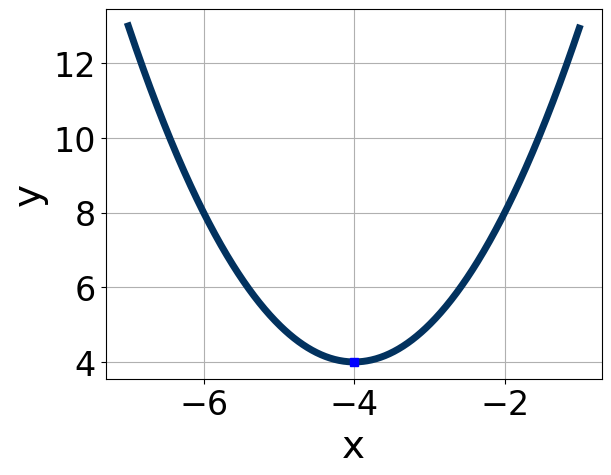
\includegraphics[width=0.5\textwidth]{../Figures/quadraticGraphToEquationCopyC.png}
\end{center}
\begin{enumerate}[label=\Alph*.]
\item \( a \in [-1.8, 0.9], \hspace*{5mm} b \in [-9, -4], \text{ and } \hspace*{5mm} c \in [-15, -11] \)
\item \( a \in [-0.6, 1.1], \hspace*{5mm} b \in [-9, -4], \text{ and } \hspace*{5mm} c \in [17, 22] \)
\item \( a \in [-0.6, 1.1], \hspace*{5mm} b \in [7, 13], \text{ and } \hspace*{5mm} c \in [17, 22] \)
\item \( a \in [-1.8, 0.9], \hspace*{5mm} b \in [7, 13], \text{ and } \hspace*{5mm} c \in [-15, -11] \)
\item \( a \in [-0.6, 1.1], \hspace*{5mm} b \in [-9, -4], \text{ and } \hspace*{5mm} c \in [12, 13] \)

\end{enumerate} }
\litem{
Graph the equation below.\[ f(x) = -(x+2)^2 + 10 \]\begin{enumerate}[label=\Alph*.]
\begin{multicols}{2}\item 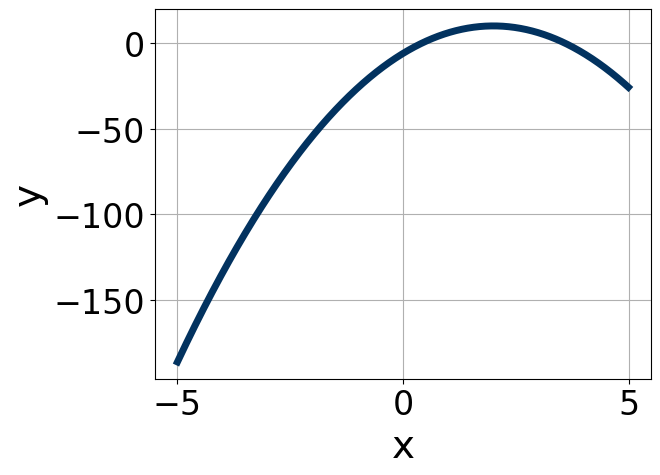
\includegraphics[width = 0.3\textwidth]{../Figures/quadraticEquationToGraphAC.png}\item 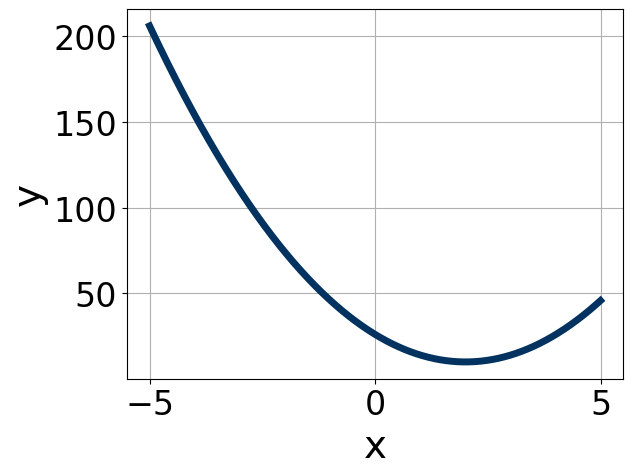
\includegraphics[width = 0.3\textwidth]{../Figures/quadraticEquationToGraphBC.png}\item 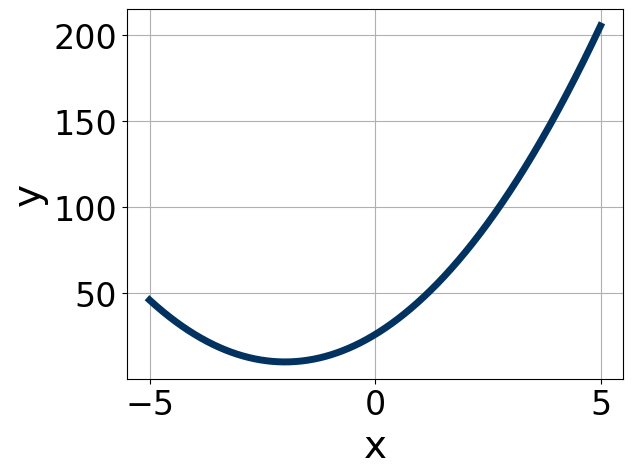
\includegraphics[width = 0.3\textwidth]{../Figures/quadraticEquationToGraphCC.png}\item 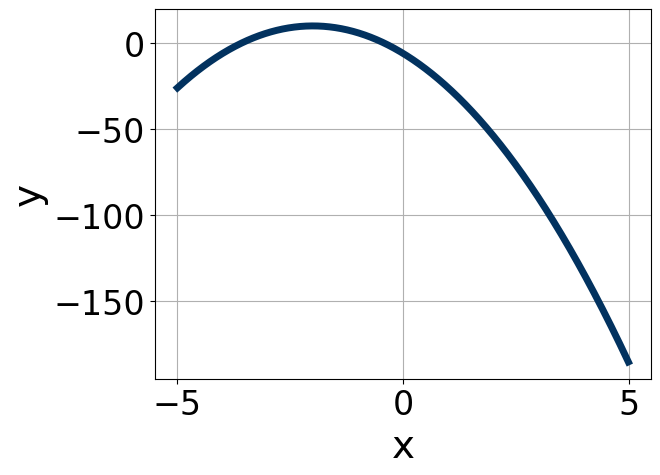
\includegraphics[width = 0.3\textwidth]{../Figures/quadraticEquationToGraphDC.png}\end{multicols}\item None of the above.
\end{enumerate} }
\litem{
Solve the quadratic equation below. Then, choose the intervals that the solutions belong to, with $x_1 \leq x_2$ (if they exist).\[ 18x^{2} +10 x -7 = 0 \]\begin{enumerate}[label=\Alph*.]
\item \( x_1 \in [-25.15, -23.62] \text{ and } x_2 \in [23.8, 26] \)
\item \( x_1 \in [-0.79, 0.13] \text{ and } x_2 \in [0.9, 1.5] \)
\item \( x_1 \in [-17.42, -17.07] \text{ and } x_2 \in [6.4, 8.4] \)
\item \( x_1 \in [-0.99, -0.95] \text{ and } x_2 \in [-0.2, 0.9] \)
\item \( \text{There are no Real solutions.} \)

\end{enumerate} }
\litem{
Solve the quadratic equation below. Then, choose the intervals that the solutions $x_1$ and $x_2$ belong to, with $x_1 \leq x_2$.\[ 20x^{2} -21 x -54 = 0 \]\begin{enumerate}[label=\Alph*.]
\item \( x_1 \in [-3.95, -3.57] \text{ and } x_2 \in [0.52, 2.17] \)
\item \( x_1 \in [-24.11, -23.57] \text{ and } x_2 \in [44.9, 46.39] \)
\item \( x_1 \in [-6.19, -5.88] \text{ and } x_2 \in [-0.33, 0.48] \)
\item \( x_1 \in [-1.76, -1.17] \text{ and } x_2 \in [2.03, 2.41] \)
\item \( x_1 \in [-0.8, 0.32] \text{ and } x_2 \in [5.83, 7.15] \)

\end{enumerate} }
\litem{
Graph the equation below.\[ f(x) = -(x-1)^2 - 13 \]\begin{enumerate}[label=\Alph*.]
\begin{multicols}{2}\item 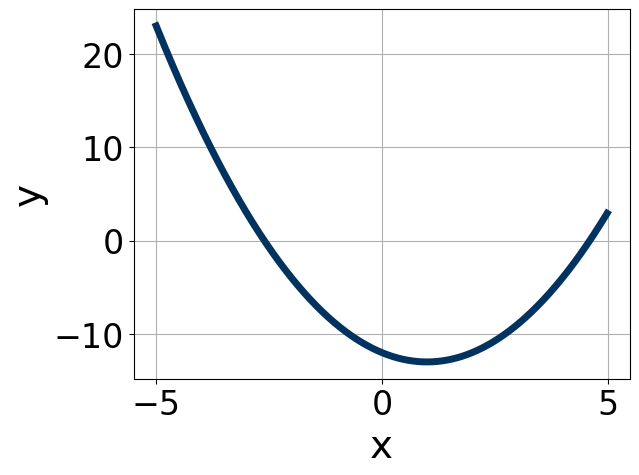
\includegraphics[width = 0.3\textwidth]{../Figures/quadraticEquationToGraphCopyAC.png}\item 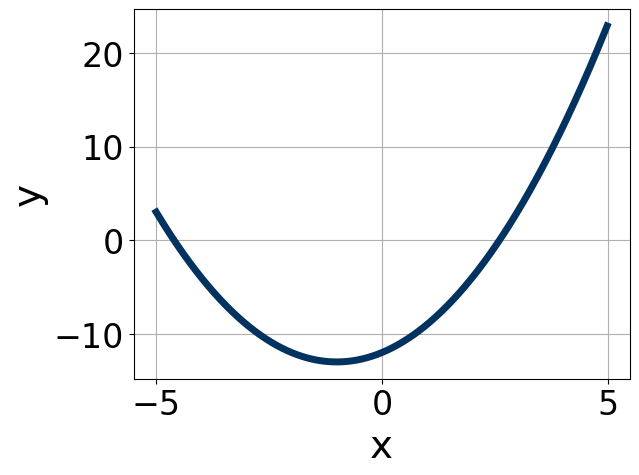
\includegraphics[width = 0.3\textwidth]{../Figures/quadraticEquationToGraphCopyBC.png}\item 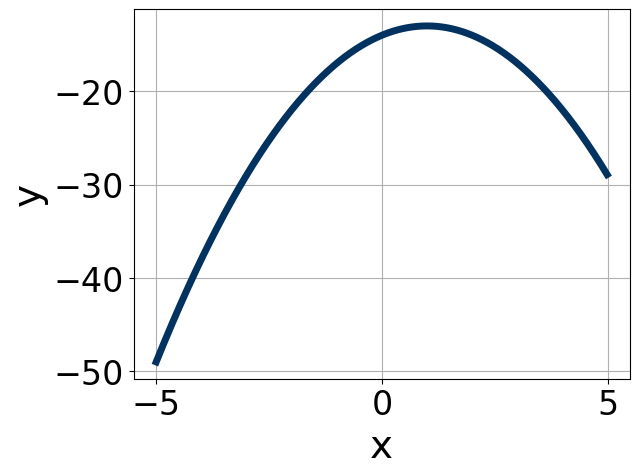
\includegraphics[width = 0.3\textwidth]{../Figures/quadraticEquationToGraphCopyCC.png}\item 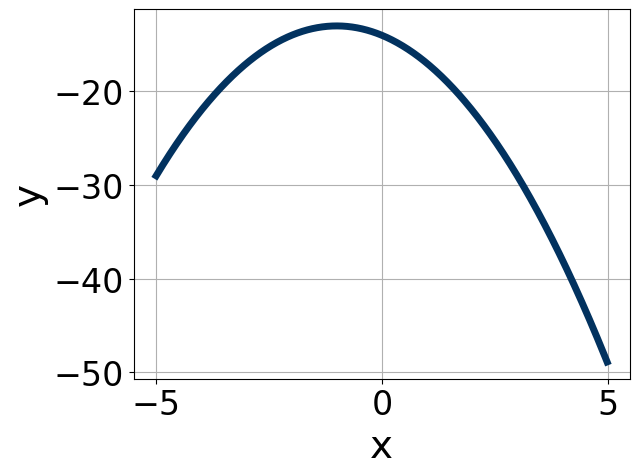
\includegraphics[width = 0.3\textwidth]{../Figures/quadraticEquationToGraphCopyDC.png}\end{multicols}\item None of the above.
\end{enumerate} }
\litem{
Solve the quadratic equation below. Then, choose the intervals that the solutions belong to, with $x_1 \leq x_2$ (if they exist).\[ 12x^{2} +12 x -7 = 0 \]\begin{enumerate}[label=\Alph*.]
\item \( x_1 \in [-0.86, 0.31] \text{ and } x_2 \in [0.8, 2.3] \)
\item \( x_1 \in [-22.76, -21.95] \text{ and } x_2 \in [21.3, 22.1] \)
\item \( x_1 \in [-1.58, -0.97] \text{ and } x_2 \in [-1.3, 0.9] \)
\item \( x_1 \in [-17.73, -16.66] \text{ and } x_2 \in [3.1, 6.8] \)
\item \( \text{There are no Real solutions.} \)

\end{enumerate} }
\litem{
Factor the quadratic below. Then, choose the intervals that contain the constants in the form $(ax+b)(cx+d); b \leq d.$\[ 36x^{2} -60 x + 25 \]\begin{enumerate}[label=\Alph*.]
\item \( a \in [-2.3, 2.1], \hspace*{5mm} b \in [-31, -29], \hspace*{5mm} c \in [0.8, 1.8], \text{ and } \hspace*{5mm} d \in [-34, -25] \)
\item \( a \in [2.9, 4], \hspace*{5mm} b \in [-5, -2], \hspace*{5mm} c \in [11.6, 13.9], \text{ and } \hspace*{5mm} d \in [-6, -2] \)
\item \( a \in [4.9, 6.6], \hspace*{5mm} b \in [-5, -2], \hspace*{5mm} c \in [3.4, 6.6], \text{ and } \hspace*{5mm} d \in [-6, -2] \)
\item \( a \in [16.9, 18.3], \hspace*{5mm} b \in [-5, -2], \hspace*{5mm} c \in [1.5, 3.2], \text{ and } \hspace*{5mm} d \in [-6, -2] \)
\item \( \text{None of the above.} \)

\end{enumerate} }
\end{enumerate}

\end{document}